\newpage
\section{Primera Parte: RTT}
\indent En esta primera parte vamos a ver como el RTT se ve afectado por el tráfico en internet, para esto realizamos pruebas en diferentes horarios y con IPs destino en diferentes partes del mundo.\\

\indent Los destinos que elegimos fueron Cambridge University (Inglaterra), Stanford University (Estados Unidos) y Moscow State University (Rusia).\\

\begin{figure}[h!]
    \centering
    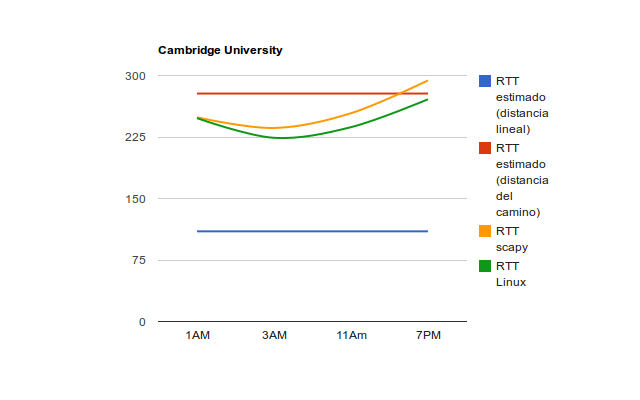
\includegraphics[width=400pt]{cambridge.png}
    \caption{Cambridge University}
    \label{fig:cambridge:count}
\end{figure}

\begin{figure}[h!]
    \centering
    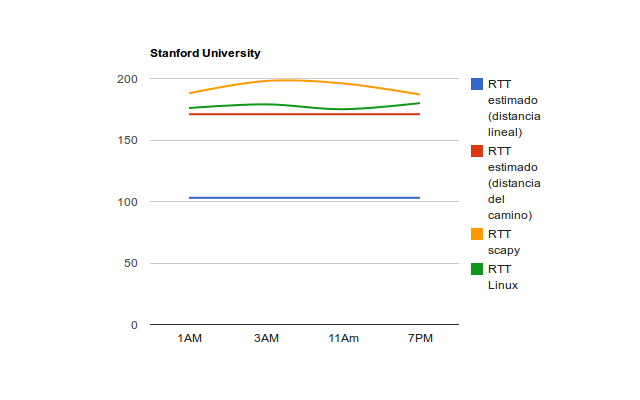
\includegraphics[width=400pt]{stanford.png}
    \caption{Stanford University}
    \label{fig:stanford:count}
\end{figure}

\begin{figure}[h!]
    \centering
    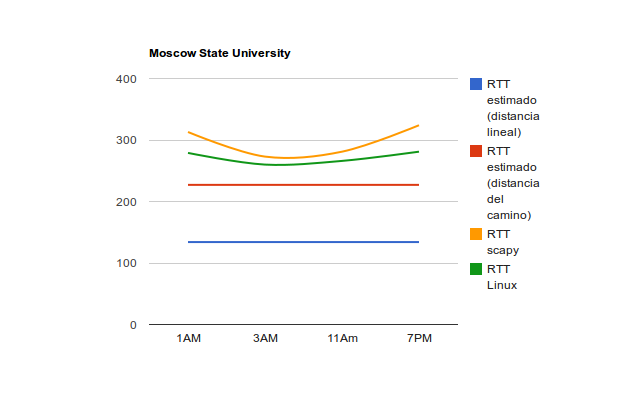
\includegraphics[width=400pt]{msu.png}
    \caption{Moscow State University}
    \label{fig:msu:count}
\end{figure}

\indent Nos pareció interesante saber cuantos km de mas tuvimos que recorrer dado que, por razones obvias, no tenemos un enlace punto a punto desde nuestras casas hacia el destino. Es por eso que están graficados ambos RTTs teóricos, creimos que tomando la distancia recorrida hasta llegar a destino iba a dar un RTT más ajustado a la realidad y así fue.\\

\indent Lo primero que se observa es como a la madrugada el RTT es menor en las dos rutas hacia Europa debido a que en ese horario el tráfico es menor tanto en el origen como en el destino, esto no sucede en la ruta hacia Estados Unidos ya que al ser en la costa oeste 4hs menos que en Buenos Aires a esa hora todavía se registra un tráfico mayor.\\

\indent En el primer gráfico llama la atención que el RTT teórico sea superior en algunos casos al RTT observado, creemos que esto se debe a un posible error en la herramienta de geolocalización ya que hay un desvío de unos 1000km en uno de los últimos hops. También puede estar sucediendo que ese hop, que tiene una IP de Escocia, en realidad sea un servidor que está en Inglaterra pero por alguna razón tiene una IP de ese país. Lo mismo sucede con uno de los primeros hops, que tiene una IP de Estados Unidos pero el RTT medido es de 28ms.\\

\indent Por último vimos que los resultados de las dos herramientas son bastante similares, probablemente el hecho de que la implementación de Traceroute del sistema operativo haga 3 intentos por hop sea la razón por la cual su curva sea más suave.\\

